\documentclass[10pt,letterpaper,spanish,twoside]{report}

\usepackage{practica}
\usepackage{graphicx}
\usepackage{float}
\DeclareGraphicsExtensions{.bmp,.png,.pdf,.jpg}
\newcommand{\docdate}{
  \vspace{2em}
   \begin{flushright}
     Ciudad de México. \datedayname~\today.
   \end{flushright}
  \vspace{2em}
}

\begin{document}
\docdate

\begin{center}
 \textsc{\asignatura}\vspace{.2em}
\end{center}

\textsc{Manual del profesor}

\textsc{Práctica 1. aplicación de filtros analógicos tipo Butterworth pasa bajas a señales biomédicas reales}

\textsc{Objetivo:} Aplicar los conocimientos sobre el diseño de filtros Butterworth pasa bajas para procesamiento de señales biomédicas reales simulando su adquisición en tiempo real

\textsc{Actividades}
\begin{enumerate}
 \item Obtener la FFT de la señal de presión sanguínea en el osciloscopio y localizar la frecuencia de corte para el filtro, en la figura 1 se puede observar que el ruido de la señal se encuentra entre las frecuencias 90 y 120 Hz.
 \\Para el diseño del filtro se creo una función que permite calcular los valores de las resistencias y capacitores con topología Sallen-Key que puede ser consultada en el archivo Diseño de filtros.ipynb\\ Se sugiere utilizar una frecuencia de corte de 70 Hz para el diseño del filtro pasa bajas orden 2
 \item Implementar el fitro que se muestra en la figura~\ref{contexto:PB2}
 \begin{figure}[H]
 	\centering
 	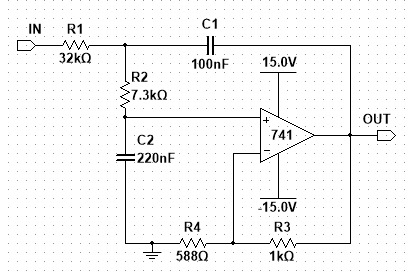
\includegraphics[scale=0.4]{PB2.PNG}
 	\caption{Circuito eléctrico de filtro pasa bajas orden 2}
	\label{contexto:PB2}
 \end{figure}
 \item En la figura~\ref{contexto:RF_2} se observa la respuesta en frecuencia del filtro
 \\Los datos obtenidos pueden consultarse en el archivo P1$\_$n2$\&$4$\_$caracterizacion.ipynb \\Es posible observar que la frecuencia de corte se encuentra en alrededor de los 62 Hz 
  \begin{figure}[H]
 	\centering
 	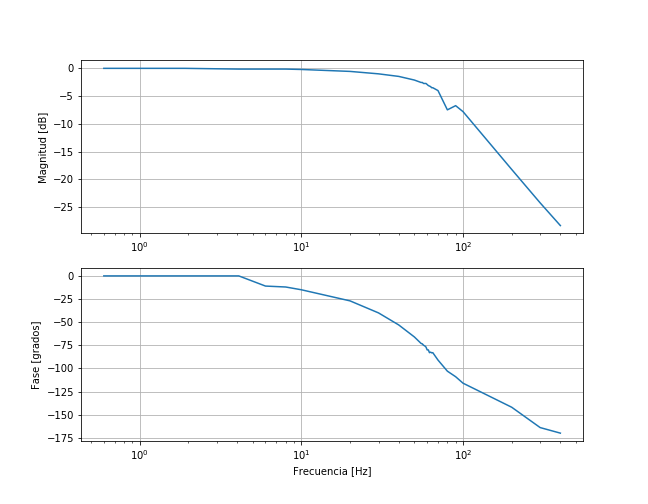
\includegraphics[scale=0.4]{RF_PB2.PNG}
 	\caption{Respuesta en frecuencia de filtro pasa bajas orden 2}
	\label{contexto:RF_2}
 \end{figure}
 \item Para el diseño del filtro pasa bajas orden 4 se sugiere utilizar una frecuencia de corte de 75Hz.
 \item Implementar circuito de la figura~\ref{contexto:PB4}
  \begin{figure}[H]
 	\centering
 	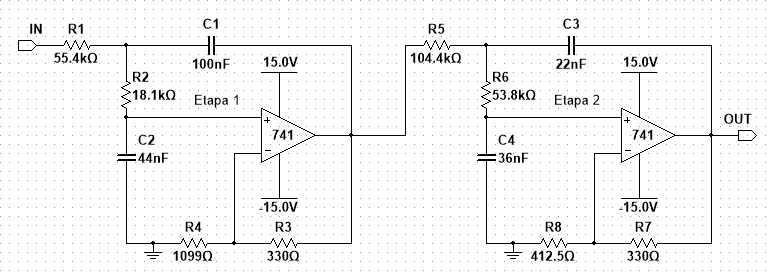
\includegraphics[scale=0.7]{PB4.PNG}
 	\caption{Circuito eléctrico de filtro pasa bajas orden 4}
	\label{contexto:PB4}
 \end{figure}
 \item En la figura~\ref{contexto:RF_4} se observa la respuesta en frecuencia del filtro pasa bajas orden 4, es posible observar que la frecuencia de corte se encuentra en alrededor de 80 Hz
 \begin{figure}[H]
 	\centering
 	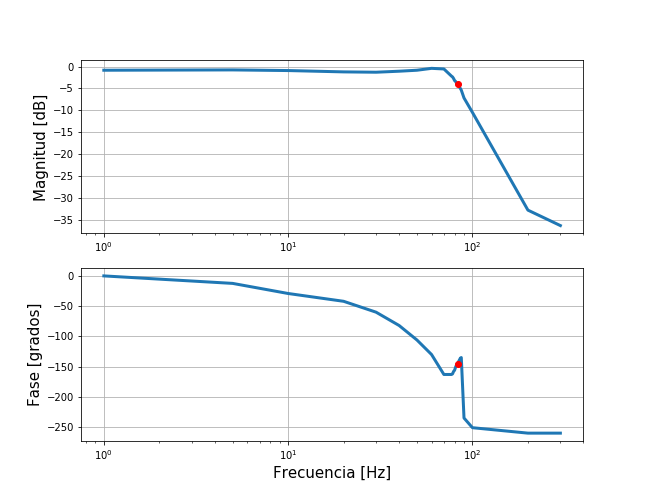
\includegraphics[scale=0.4]{RF_PB4.PNG}
 	\caption{Respuesta en frecuencia de filtro pasa bajas orden 4}
	\label{contexto:RF_4}
 \end{figure}
 \item Para probar el funcionamiento de dichos filtros, es necesario observar que la señal de presión sanguínea se vea correctamente filtrada con ayuda del osciloscopio
\end{enumerate}


%\textsc{Nota}
%\vspace{2em}
\vfill
\begin{flushright}
\textsc{Elaboró:\\
Ma. del Rosario Aguilar Cruz\\
Enrique Mena Camilo}
\end{flushright}

\end{document}